\documentclass[]{beamer}  % only frames

\usepackage{amsmath,amssymb,amsfonts}
\usepackage{array}
\usepackage[british]{babel}
\usepackage{bbm}
\usepackage{bbold}
\usepackage{beamerthemesplit}
\usepackage[bf]{caption}
\usepackage{cite}
\usepackage{color}
\usepackage{enumerate}
\usepackage{eurosym}
\usepackage{graphicx}
\usepackage{rotating}
\usepackage{slashed}
\usepackage[utf8]{luainputenc}
\usepackage{xcolor}
\usepackage{array}
\usepackage{listings}
\usepackage{nicefrac} % for \nicefrac macro giving nice fractions in exponent
\usepackage{enumerate}

\usepackage{pgfplots}
\pgfplotsset{compat=1.10}

% For table:
% ----------
\usepackage{color}
\usepackage{colortbl}
\usepackage{multirow}
\usepackage[makeroom]{cancel} % needed for xcancel

% My fonts:
% ---------
\usepackage{libertine}
% \usepackage{tgcursor}
\usefonttheme[onlymath]{serif}
\usepackage[activate]{microtype}

% My definitions:
% ---------------
\newcommand\TTspace{ 0pt }
\newcommand\TT{ \scriptscriptstyle{\mathrm{T\hspace{\TTspace}T}} }
\newcommand\hTT{ h_{\scriptscriptstyle{\mathrm{T\hspace{\TTspace}T}}} }
\newcommand\NS{ N_{\scriptscriptstyle{\mathrm{S}}} }
\newcommand\GNewton{ G_{\scriptscriptstyle{\mathrm{N}}}{} }
\newcommand\SEH{ S_{\scriptscriptstyle{\mathrm{EH}}}{} }
\newcommand\SUV{ S_{\scriptscriptstyle{\mathrm{UV}}}{} }
\newcommand\Sbare{ S_{\scriptscriptstyle{\mathrm{bare}}}{} }
\newcommand\Sclass{ S_{\scriptscriptstyle{\mathrm{classical}}}{} }
\newcommand\MPl{ M_{\scriptscriptstyle{\mathrm{Pl}}}{} }
\newcommand\metric{ g_{\mu\nu} }
\newcommand{\weyl}{\delta_\varepsilon}

\newcommand{\overbar}[1]{\mkern 1.5mu\overline{\mkern-1.5mu#1\mkern-1.5mu}\mkern 1.5mu}
\newcommand{\bnabla}{\overbar \nabla}
\newcommand\etaS{ \eta_{\scriptscriptstyle{\mathrm{S}}} }
\newcommand\etaTT{ \eta_{\scriptscriptstyle{\mathrm{T\hspace{\TTspace}T}}} }

\newcommand{\FPone}  {\textbf{FP1}}
\newcommand{\FPtwo}  {\textbf{FP2}}

%----------------------------------------------------------------------------------------
% TikZ & PGFPLOTS SETUP (FOR PLOTTING IN LATEX)
%----------------------------------------------------------------------------------------

\usepackage{tikz}
\usepackage{pgfplots}
\usepackage{pgfplotstable}
\pgfplotsset{compat=newest}

\usepackage{graphicx}
\usepackage[dvipsnames]{xcolor}
\usepackage{scalerel}

\usetikzlibrary{patterns}
\usetikzlibrary{matrix}
\usetikzlibrary{positioning}
\usetikzlibrary{arrows.meta}
\usetikzlibrary{fit}
\usetikzlibrary{math}
\usetikzlibrary{calc}
\usetikzlibrary{backgrounds}
\usetikzlibrary{decorations.pathmorphing}
\usetikzlibrary{decorations.markings}
\usetikzlibrary{pgfplots.groupplots}

\tikzset{
  midarrow/.style={draw, postaction={decorate},
  decoration={markings,mark=at position .55 with {\arrow[draw]{>}}}},
  midarrow-rev/.style={draw, postaction={decorate},
  decoration={markings,mark=at position .55 with {\arrow[draw]{<}}}},
  midarrow-dashed/.style={draw, dashed, postaction={decorate},
  decoration={markings,mark=at position .55 with {\arrow[draw]{>}}}},
  midarrow-dashed-thick/.style={
    draw, thick, dashed, postaction={decorate},
  decoration={markings,mark=at position .50 with {\arrow[draw]{>}}}},
}
\tikzset{
  TT/.style={decorate, draw=black,
  decoration={coil,aspect=0.7,segment length=3.2pt,amplitude=2pt}}
}
\tikzset{
  sigma/.style={dashed}
}

\usepgfplotslibrary{groupplots} % Libraries to generate group plots
%----------------------------------------------------------------------------------------
% OTHER STUFF
%----------------------------------------------------------------------------------------

\newsavebox\bracebox

\makeatletter
\def\amsbb{\use@mathgroup \M@U \symAMSb}
\makeatother

\usetheme{Boadilla}

\setbeamertemplate{section in toc}[sections numbered]
\setbeamertemplate{blocks}[rounded][shadow=false]
\setbeamertemplate{itemize items}[default]
\beamertemplatenavigationsymbolsempty
\setbeamercolor{footline}{bg=black}
\setbeamertemplate{footline}{%
  \raisebox{8pt}{\makebox[\paperwidth]{\hfill\makebox[15pt]{{\tiny\insertframenumber}}\qquad}}
}

\definecolor{myred}{RGB}{176,50,50}
\definecolor{myblue}{RGB}{50,50,176}
\definecolor{mygreen}{RGB}{60,166,60}

\newcommand\blfootnote[1]{%
  \begingroup
    \renewcommand\thefootnote{}\footnote{#1}%
    \addtocounter{footnote}{-1}%
    \endgroup
}

%----------------------------------------------------------------------------------------
% DOCUMENT
%----------------------------------------------------------------------------------------

\begin{document}

% General TODO:
% More colour everywhere!

%%%%%%%%%%%%%%%%%%%%%%%%%%%%%%%%%%%%%%%%%%
%%%   TITLE SLIDE
%%%%%%%%%%%%%%%%%%%%%%%%%%%%%%%%%%%%%%%%%%

\title{Matter fields in the Asymptotic Safety scenario}
\author{Peter Labus}
\institute{SISSA Trieste
  \vspace{5mm}
  \\ \vspace{8pt}P.L., T. R. Morris and Z. H. Slade, Phys. Rev. D 94 (2016)
  \\ \vspace{8pt}P. Don\`a, A. Eichhorn, P.L. and R. Percacci, Phys. Rev. D93 (2016)
  \\ \vspace{8pt}P.L., R. Percacci, G.P. Vacca, Phys. Lett.  B753 (2016)
  \\ \vspace{8pt}A. Eichhorn, P.L., J. M. Pawlowski, M. Reichert, \textit{In preparation.}
  \date{14/09/2017}
}
\begin{frame}[noframenumbering,plain]
  \titlepage
\end{frame}

%----------------------------------------------------------------------------------------
%   Section 1 --- Quantum Gravity
%----------------------------------------------------------------------------------------

\section{Asymptotically safe quantum gravity}
\fontsize{10pt}{7.2}\selectfont

%%%%%%%%%%%%%%%%%%%%%%%%%%%%%%%%%%%%%%%%%%
%%%   SLIDE 1
%%%%%%%%%%%%%%%%%%%%%%%%%%%%%%%%%%%%%%%%%%

% TODO:

\begin{frame}
  \frametitle{Outline}
  \begin{enumerate}[I]
    \item
      Asymptotic Safety
      \begin{itemize}
        \item Why quantum gravity?
        \item What is asymptotic safety and why to study it?
      \end{itemize}
      \vfill
    \item
      Matter fields coupled to gravity
      \begin{itemize}
        \item Why we should include matter fields from the start...
        \item ...and what we might learn from it
      \end{itemize}
      \vfill
    \item
      Tools to study asymptotic safety
      \begin{itemize}
        \item What is needed and available?
        \item Why to use the functional renormalisation group (FRG)?
      \end{itemize}
      \vfill
    \item
      Known issues of the FRG in gravity
      \begin{itemize}
        \item Outline of some open research questions...
        \item ...and relation to my own work
      \end{itemize}
      \vfill
    \item
      My research \& its implications
  \end{enumerate}
\end{frame}

%%%%%%%%%%%%%%%%%%%%%%%%%%%%%%%%%%%%%%%%%%
%%%   SLIDE 2
%%%%%%%%%%%%%%%%%%%%%%%%%%%%%%%%%%%%%%%%%%

% TODO:
% consistent spacing
% maybe only one question on last version of slide

\begin{frame}
  \frametitle{Why quantum gravity?}
  \textbf{Two pressing issues:}
  \begin{enumerate}
    \item singularities in GR (black holes, big bang)
      \hspace{2cm}
      \raisebox{-.5\height}{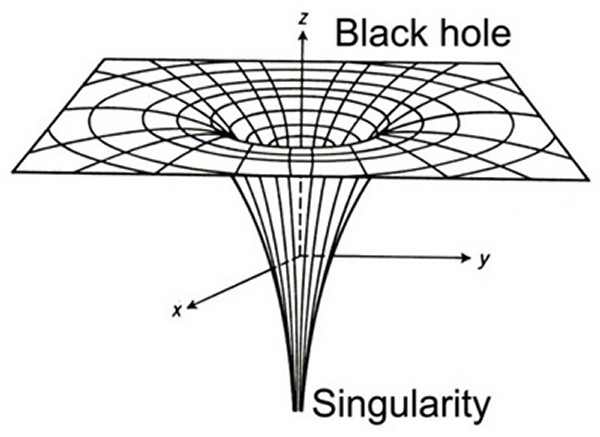
\includegraphics[width=0.25\textwidth]{blackholes_singularity.jpg}}
    \item singularities in SM (stability of $U(1)_Y$ and Higgs sector)
      % \hspace{1cm}
      \raisebox{-.5\height}{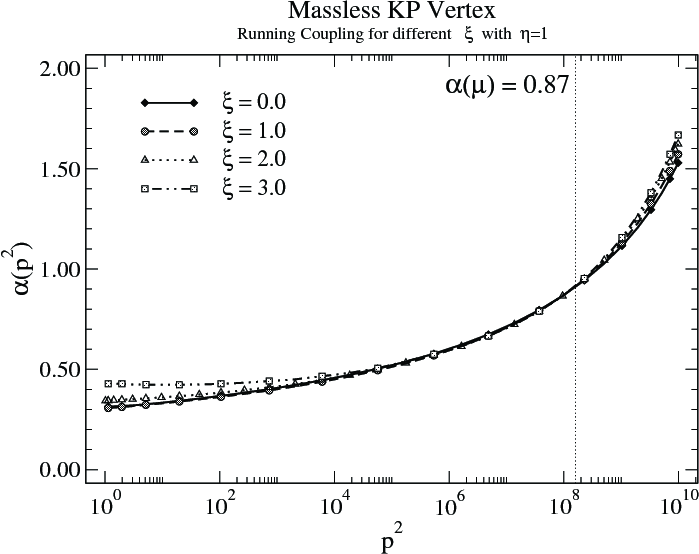
\includegraphics[width=0.25\textwidth]{running_alpha.png}}
  \end{enumerate}
  \vfill
  \pause
  \textbf{More theoretical issues:}\\[5pt]
  cosmological constant problem, hierarchy problem, origin of symmetries and field content,
  CP-violation, grand unification?, TOE?, \dots
\end{frame}

\addtocounter{framenumber}{-1}
\begin{frame}
  \frametitle{Why quantum gravity?}
  \textbf{Two pressing issues:}
  \begin{enumerate}
    \item singularities in GR (black holes, big bang)
      \hspace{2cm}
      \raisebox{-.5\height}{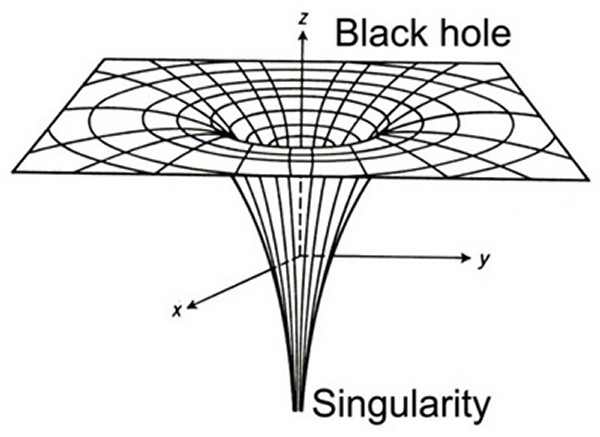
\includegraphics[width=0.25\textwidth]{blackholes_singularity.jpg}}
    \item singularities in SM (stability of $U(1)$ and Higgs sector)
      % \hspace{1cm}
      \raisebox{-.5\height}{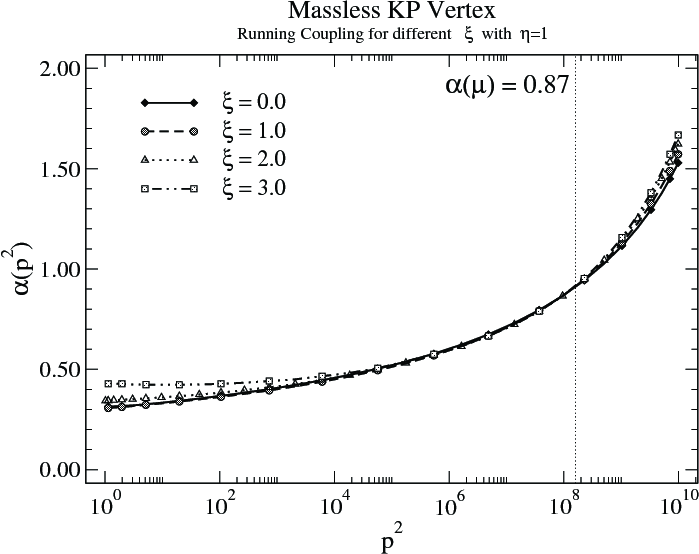
\includegraphics[width=0.25\textwidth]{running_alpha.png}}
  \end{enumerate}
  \vfill
  \begin{center}
    \fontsize{12pt}{7.2}\selectfont
    \textbf{ Can one help to cure the other? }
    \raisebox{-.5\height}{
\includegraphics[width=0.25\textwidth]{two_birds.jpg}}
  \end{center}
  \pause
  \begin{center}
    candidates:\\[5pt]
    string theory, loop quantum gravity, causal dynamical triangulation, Regge calculus,\\
    causal sets, spin foams, group field theory, \dots
  \end{center}
\end{frame}

\addtocounter{framenumber}{-1}
\begin{frame}
  \frametitle{Why quantum gravity?}
  \textbf{Two pressing issues:}
  \begin{enumerate}
    \item singularities in GR (black holes, big bang)
      \hspace{2cm}
      \raisebox{-.5\height}{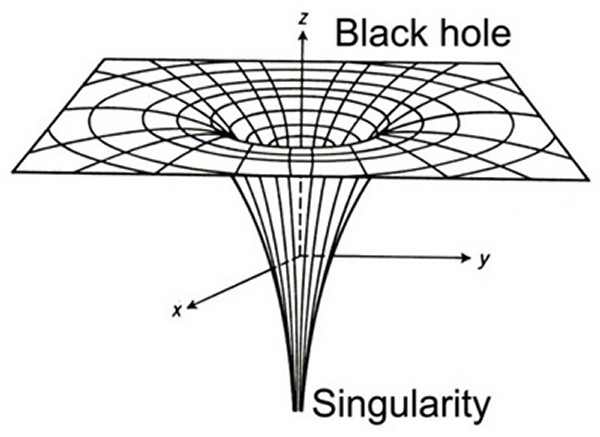
\includegraphics[width=0.25\textwidth]{blackholes_singularity.jpg}}
    \item singularities in SM (stability of $U(1)$ and Higgs sector)
      % \hspace{1cm}
      \raisebox{-.5\height}{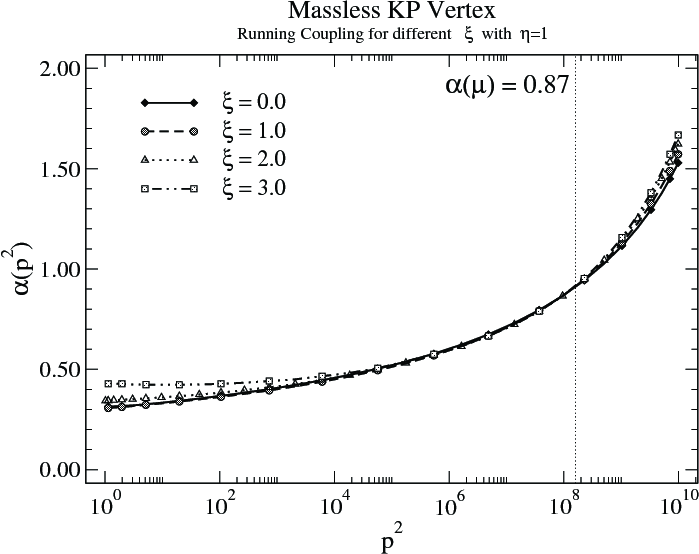
\includegraphics[width=0.25\textwidth]{running_alpha.png}}
  \end{enumerate}
  \vfill
  \begin{center}
    \fontsize{12pt}{7.2}\selectfont
    \textbf{ Can one help to cure the other? } \\[15pt]
    \textbf{ Have to go beyond QFTs? }
  \end{center}
\end{frame}

%%%%%%%%%%%%%%%%%%%%%%%%%%%%%%%%%%%%%%%%%%
%%%   SLIDE 3
%%%%%%%%%%%%%%%%%%%%%%%%%%%%%%%%%%%%%%%%%%

% TODO:
% references
% check formula
% Feynman diagram of graviton scattering
% picture of Einstein?

\begin{frame}
  \frametitle{But wait a minute...!}
  \textbf{We know (low-energy) quantum gravity:}\\[5pt]
  GR as an EFT $\rightarrow$ can calculate corrections to Newtonian potential [Donogue et al.]
  \begin{align*}
    \boxed{
      V(r) = -\frac{\GNewton m_1 m_2}{r}
      \bigg(
        1
        + 3 \, \frac{\GNewton (m_1 + m_2)}{r \, c^2}
        + \frac{41}{10 \pi} \, \frac{\GNewton \hbar}{r^2 \, c^3}
        + \dots
      \bigg)
    }
  \end{align*}
  \hfill Probably most accurate result in quantum gravity...!
  \pause
  \vfill
  \begin{itemize}
    \item well-defined QFT of gravity\\[5pt]
    \item predictive, but experimentally indistinguishable from GR\\[5pt]
    \item consistent with all available data
  \end{itemize}
\end{frame}

\addtocounter{framenumber}{-1}
\begin{frame}
  \frametitle{But wait a minute...!}
  \textbf{We know (low-energy) quantum gravity:}\\[5pt]
  GR as an EFT $\rightarrow$ can calculate corrections to Newtonian potential [Donogue et al.]
  \begin{align*}
    \boxed{
      V(r) = -\frac{\GNewton m_1 m_2}{r}
      \bigg(
        1
        + 3 \, \frac{\GNewton (m_1 + m_2)}{r \, c^2}
        + \frac{41}{10 \pi} \, \frac{\GNewton \hbar}{r^2 \, c^3}
        + \dots
      \bigg)
    }
  \end{align*}
  \hfill Probably most accurate result in quantum gravity...!
  \pause
  \vfill
  \begin{center}
    \fontsize{12pt}{7.2}\selectfont
    \textbf{ So, what's the catch? }
  \end{center}
  \pause
  \vspace{10pt}
  Expansion in $\nicefrac{k}{\MPl}$ needs $\infty$--terms in UV:\\[5pt]
  \begin{itemize}
    \item How to make predictions at the Planck scale?\\[5pt]
    \item Can we address either of our two issues?
  \end{itemize}
\end{frame}

%%%%%%%%%%%%%%%%%%%%%%%%%%%%%%%%%%%%%%%%%%
%%%   SLIDE 4
%%%%%%%%%%%%%%%%%%%%%%%%%%%%%%%%%%%%%%%%%%

% TODO:
% picture Feynman?

\begin{frame}
  \frametitle{The path integral approach}
  % \textbf{Have to make sense of}
  \begin{align*}
    \boxed{
    \int \mathcal D \Phi \; e^{i S[\Phi]}\,,
    \text{ let's try } \Phi = \metric \,.
    }
  \end{align*}
  \vfill
  % Have to specify:
  \begin{itemize}
    \item integration measure $\mathcal D \metric$ (integral over all space-times)
    \item action $S[\metric]$
  \end{itemize}
  \vfill
  \begin{enumerate}
    \item $S[\metric] = \SEH[\metric] = - \frac{1}{16 \pi \GNewton} \int \sqrt{g} \, R$
      \hspace{2pt}
      \textit{does not work} [t'Hooft, Veltman]\\[15pt]
    \item $S = \Sbare = \SUV = \, ???\,,$\\[5pt]
          $S \neq \Sclass$
  \end{enumerate}
\end{frame}

\addtocounter{framenumber}{-1}
\begin{frame}
  \frametitle{The path integral approach}
  % \textbf{Have to make sense of}
  \begin{align*}
    \boxed{
    \int \mathcal D \Phi \; e^{i S[\Phi]}\,,
    \text{ let's try } \Phi = \metric \,.
    }
  \end{align*}
  \vfill
  % Have to specify:
  \begin{itemize}
    \item integration measure $\mathcal D \metric$ (integral over all space-times)
    \item action $S[\metric]$
  \end{itemize}
  \vfill
  \begin{center}
    \fontsize{12pt}{7.2}\selectfont
    \textbf{ What is going wrong here? }
  \end{center}
  \begin{columns}[T]
    \begin{column}{.5\textwidth}
      \begin{center}
        couplings of the theory are \textbf{scale-dependent},\\[10pt]
        na\"ively $\GNewton \rightarrow \infty$ in the UV limit
      \end{center}
    \end{column}
    \begin{column}{.5\textwidth}
      \begin{center}
        vacuum polarisation in QED:
        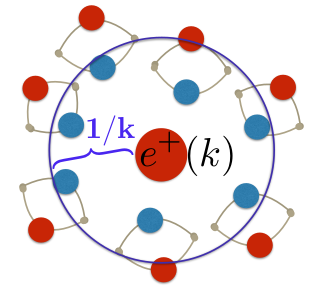
\includegraphics[width=0.4\textwidth]{screening.png}
      \end{center}
    \end{column}
  \end{columns}
\end{frame}

%%%%%%%%%%%%%%%%%%%%%%%%%%%%%%%%%%%%%%%%%%
%%%   SLIDE 5
%%%%%%%%%%%%%%%%%%%%%%%%%%%%%%%%%%%%%%%%%%

% TODO:

\begin{frame}
  \frametitle{A look into theory space}
  scale-dependent \textbf{effective average action}
  \begin{align*}
    \boxed{
    e^{ - \Gamma_k \lbrack \varphi \rbrack }
    = \int \mathcal D \chi \;
    e^{
      - S \lbrack \chi + \varphi \rbrack
      - \Delta S_k \lbrack \chi \rbrack
      + \int \mathrm d^dx \;
      \frac{ \delta \Gamma_k }{ \delta \varphi (x) }
      \, \chi(x)
    }
    }
  \end{align*}
  \vspace{2pt}

  \begin{columns}[T]
    \begin{column}{.4\textwidth}
      \textbf{Theory space:}\\[5pt]
      QFT = trajectory in theory space,
      parametrised by scale $k$\\[25pt]
      % \begin{center}
        \includegraphics[scale=0.6]{theory_space.pdf}
      % \end{center}
    \end{column}
    \begin{column}{.6\textwidth}
      \begin{center}
        $\Gamma_k \lbrack \varphi \rbrack = \sum_n \, g_n(k) \; \mathcal O_n(\varphi, \partial)$\\[5pt]
        all operators allowed by symmetry\\[3pt]
        (generated by quantum fluctuations)\\[20pt]
        \pause
        \textbf{Q:} All $g_n(k)<\infty$ for all $k$?\\[5pt]
        \textbf{A:} Ultra violet \textbf{fixed point}!
      \end{center}
    \end{column}
  \end{columns}
\end{frame}

\addtocounter{framenumber}{-1}
\begin{frame}
  \frametitle{A look into theory space}
  \vspace{7.5pt}
  scale-dependent \textbf{effective average action}
  \begin{align*}
    \boxed{
    e^{ - \Gamma_k \lbrack \varphi \rbrack }
    = \int \mathcal D \chi \;
    e^{
      - S \lbrack \chi + \varphi \rbrack
      - \Delta S_k \lbrack \chi \rbrack
      + \int \mathrm d^dx \;
      \frac{ \delta \Gamma_k }{ \delta \varphi (x) }
      \, \chi(x)
    }
    }
  \end{align*}
  \vspace{2pt}

  \begin{columns}[T]
    \begin{column}{.6\textwidth}
        UV critical surface:\\[10pt]
      % \begin{center}
        \includegraphics[scale=0.6]{uvcritsurface_talk.pdf}
      % \end{center}
    \end{column}
    \begin{column}{.4\textwidth}
      \begin{center}
        fixed point in $\infty$--dim\\ theory space:\\
        \textbf{asymptotic safety} (freedom)\\[20pt]
        relevant directions\\[3pt]
        $\rightarrow$ free parameters (fix in the IR)\\[10pt]
        irrelevant directions\\[3pt]
        $\rightarrow$ predictions of the theory
      \end{center}
    \end{column}
  \end{columns}
\end{frame}

%%%%%%%%%%%%%%%%%%%%%%%%%%%%%%%%%%%%%%%%%%
%%%   SLIDE 6
%%%%%%%%%%%%%%%%%%%%%%%%%%%%%%%%%%%%%%%%%%

% TODO:
% add plot G(k) over k/\mu

\begin{frame}
  \frametitle{Asymptotically safe (pure) gravity }

  \begin{columns}[T]
    \begin{column}{.6\textwidth}
      \begin{center}
        $\varepsilon$--expansion in $d=2+\epsilon$:
        \begin{align*}
          \boxed{
            \beta_G = \varepsilon \, G - \frac{38}{3} \, G^2
          }
        \end{align*}
        fixed point at positive $G_\star > 0$, classical
        and quantum scaling balance out [Weinberg `76]
      \end{center}
    \end{column}
    \begin{column}{.4\textwidth}
      \begin{center}
        % \vspace{-20pt}
        \begin{tikzpicture}[
    >=stealth,
    scale=0.50,
    thick
  ]

  \begin{axis}[
    width=5.0cm,
    height=5.0cm,
    scale only axis,
    major tick length=2pt,
    xlabel={$G$},
    ylabel={$\beta_G$},
    % xlabel shift=-7pt,
    % ylabel shift=-7pt,
    xmin=-0.0, xmax=2.1,
    ymin=-1.5, ymax=1.5,
    % xtick={0,2},
    % ytick={-2,0,2},
    ticks=none,
    legend cell align=left,
    legend pos=outer north east,
    ]

    % \addplot[blue,  domain=0:1.414, thick, ]{ x^2 };
    % \addplot[green, domain=0:1.414, thick, ]{ - x^2 };
    \addplot[red,   domain=0:2.1, thick, ]{ 2*x - x^2 };
    \addplot[black, domain=-0.1:2.1, line width=0mm,  ]{ 0 };

    % \legend{
    %   IR-GFP,
    %   UV-GFP,
    %   IR-GFP + UV-NGFP
    % }


    \node (gfp) at (axis cs:0.25,-1.0) [anchor=north] {\footnotesize GFP};
    \draw[->] (gfp) -- (axis cs:0.03,-0.1);

    \node (ngfp) at (axis cs:1.75,-1.0) [anchor=north] {\footnotesize NGFP};
    \draw[->] (ngfp) -- (axis cs:1.97,-0.1);

  \end{axis}


\end{tikzpicture}

      \end{center}
    \end{column}
  \end{columns}

  \begin{columns}[T]
    \begin{column}{.4\textwidth}
      \begin{center}
        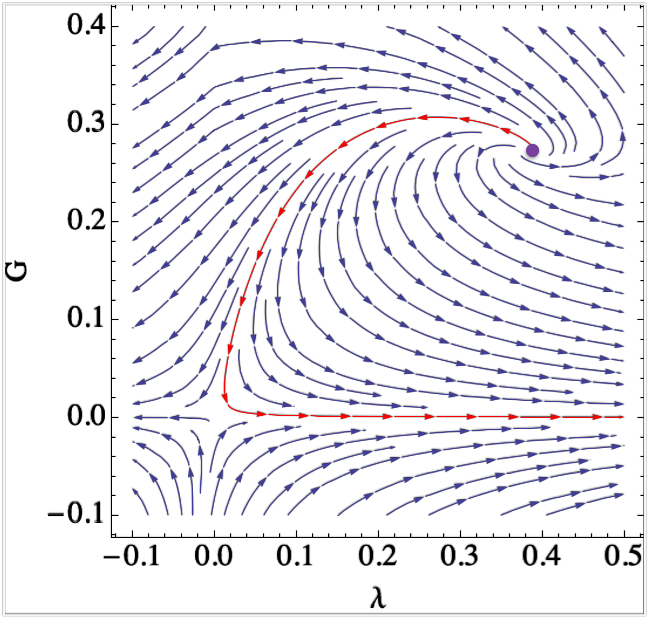
\includegraphics[width=0.9\textwidth]{fixed_point_EH.png}
      \end{center}
    \end{column}
    \begin{column}{.6\textwidth}
      \begin{center}
        Strong evidence for existence of \textbf{interacting UV FP}
        with 3 relevant directions from \textbf{functional RG}\\[5pt]
        \hfill [Reuter `96]

        \vspace{15pt}
        scale invariant UV theory flows to Einstein-Hilbert regime in IR,
        finite number of free parameters\\[5pt]
        % \vspace{5pt}
        \hfill [Reuter, Saueressig, Litim, Codello, Percacci,\\
        \hfill Rahmede, Dietz, Morris, Eichhorn, ...]
      \end{center}
    \end{column}
  \end{columns}

\end{frame}

%%%%%%%%%%%%%%%%%%%%%%%%%%%%%%%%%%%%%%%%%%
%%%   SLIDE 7
%%%%%%%%%%%%%%%%%%%%%%%%%%%%%%%%%%%%%%%%%%

% TODO:

\begin{frame}
  \frametitle{Including matter...}

\end{frame}

%%%%%%%%%%%%%%%%%%%%%%%%%%%%%%%%%%%%%%%%%%
%%%   SLIDE 8
%%%%%%%%%%%%%%%%%%%%%%%%%%%%%%%%%%%%%%%%%%

% TODO:

\begin{frame}
  \frametitle{Matter matters}

\end{frame}

%%%%%%%%%%%%%%%%%%%%%%%%%%%%%%%%%%%%%%%%%%
%%%   SLIDE
%%%%%%%%%%%%%%%%%%%%%%%%%%%%%%%%%%%%%%%%%%

% TODO:

\begin{frame}
  \frametitle{The exact renormalisation group equation}

  \begin{center}
    \textbf{
      Need non-perturbative tool for strongly interacting regime $\mathbf{g>1}$
    }
  \end{center}

  Introduce scale-dependent \textbf{effective average action}
  \begin{align*}
    e^{ - \Gamma_k \lbrack \varphi \rbrack }
    = \int \mathcal D \chi \;
    e^{
      - S \lbrack \chi + \varphi \rbrack
      - \Delta S_k \lbrack \chi \rbrack
      + \int \mathrm d^dx \;
      \frac{ \delta \Gamma_k }{ \delta \varphi (x) }
      \, \chi(x)
    } \,, \;\;
   \Delta S_k \lbrack \chi \rbrack =
   \frac 12 \int \chi(-p) R_k(p) \chi(p)
  \end{align*}
  through cutoff-operator $R_k$ (scale and momentum-dependent mass term)

  \vspace{30pt}
  \begin{columns}[T]
    \begin{column}{.5\textwidth}
      \textbf{Exact RG equation:}\\[3pt]
      \begin{align*}
        \boxed{
          \partial_t \Gamma_k
          = \frac 12 \; \mathrm{Tr}
          \left[
            \left(
              \frac{ \delta^2 \Gamma_k }{ \delta \varphi \, \delta \varphi } + R_k
            \right) ^{\!\!-1}
            \! \dot R_k
          \right]
        }
      \end{align*}
      \hfill [Wetterich `93, Morris `94]
    \end{column}
    \begin{column}{.5\textwidth}
      % \begin{center}
        \textbf{
          $\mathbf{\Gamma_k}$ contains quantum fluctuations above $\mathbf{k}$
        }\\[10pt]

        IR limit ($k \rightarrow 0$): full effective action $\Gamma$\\[5pt]
        UV limit ($k \rightarrow \infty$): UV action $S$\\
        % $\rightarrow$
        \hfill (prediction of the theory)
      % \end{center}
    \end{column}
  \end{columns}
\end{frame}

%%%%%%%%%%%%%%%%%%%%%%%%%%%%%%%%%%%%%%%%%%
%%%   SLIDE
%%%%%%%%%%%%%%%%%%%%%%%%%%%%%%%%%%%%%%%%%%

% TODO:

\begin{frame}
  \frametitle{Truncating the functional RG}

  \vspace{-33pt}
  Practical calculations: include only proper subset of all possible operators
  \begin{align*}
    \boxed{
      \Gamma_k[\Phi] = \sum_i \; g_i(k) \! \int \mathrm d^d x \; \mathcal O_i [\Phi(x)]
    }
  \end{align*}

  \vspace{-15pt}
  \begin{columns}[T]

    \begin{column}{.5\textwidth}
      \begin{center}
        \textbf{derivative expansion:}\\
        (expand in powers of momentum)
        \begin{align*}
          \Gamma_k [\Phi] &=
          \int \mathrm d^dx
          \bigg[
            V_k (\Phi)\\
            &+ \frac 12 \, Z_k (\Phi) \big( \partial_\mu \Phi \, \partial^\mu \Phi \big)\\
            &+ \frac 12 \, W_k (\Phi) \big( \Box \Phi \, \Box \Phi \big)
            + \dots
          \bigg]
        \end{align*}
      \end{center}
    \end{column}

    \begin{column}{.5\textwidth}
      \begin{center}
        \textbf{vertex expansion:}\\
        (functional Taylor expansion)
        \begin{align*}
          \Gamma_k [\Phi] =
          \sum_{n=0}^{N} \; \frac{1}{n!}
          \int \mathrm d^dx_1
          \int \mathrm d^dx_2
          \; \dots \\
          \times \int \mathrm d^dx_n \;
          \Gamma_{x_1 x_2 \dots x_n}^{(n)} \,
          \prod_{i=1}^n
          \big( \Phi(x_i) - \overbar\Phi(x_i) \big)
        \end{align*}
      \end{center}
    \end{column}

  \end{columns}
\end{frame}

\addtocounter{framenumber}{-1}
\begin{frame}
  \frametitle{Truncating the functional RG}

  Practical calculations: include only proper subset of all possible operators
  \begin{align*}
    \boxed{
      \Gamma_k[\Phi] = \sum_i \; g_i(k) \! \int \mathrm d^d x \; \mathcal O_i [\Phi(x)]
    }
  \end{align*}

  \vspace{-15pt}
  \begin{columns}[T]

    \begin{column}{.5\textwidth}
      \begin{center}
        \textbf{derivative expansion:}
        \begin{itemize}
          \item
            expanded in diffeomorphism invariant quantities
            ($R$, $R_{\mu\nu}$, $C_{\mu\nu}$, ...)\\[8pt]
          \item
            background field approximation + heat kernel
            techniques\\[8pt]
          \item
            using curved backgrounds\\
            $\rightarrow$ physically most relevant?\\[8pt]
          \item
            functional truncations\\
            $\rightarrow$ $\infty$-many operators\\[8pt]
          \item
            $\beta_{\GNewton}$ receives contributions
            from cutoff--operator\\[8pt]
        \end{itemize}
      \end{center}
    \end{column}

    \begin{column}{.55\textwidth}
      \begin{center}
        \textbf{vertex expansion:}
        \begin{itemize}
          \item
            local, non-diffeomorphism invariant action $\Gamma_k$\\
            $\rightarrow$ but maybe \textit{``effective universality''}?\\[8pt]
          \item
            calculate Feynman diagrams\\[8pt]
          \item
            many different ``avatars'' of $\GNewton$\\[8pt]
          \item
            (usually) evaluated on flat background\\
            $\rightarrow$ farther from ``true vacuum''?\\[8pt]
          \item
            functional truncations difficult\\[8pt]
          \item
            fluctuation field couplings do not receives contributions
            from cutoff--operator\\[8pt]
        \end{itemize}
      \end{center}
    \end{column}

  \end{columns}
\end{frame}

%%%%%%%%%%%%%%%%%%%%%%%%%%%%%%%%%%%%%%%%%%
%%%   SLIDE
%%%%%%%%%%%%%%%%%%%%%%%%%%%%%%%%%%%%%%%%%%

% TODO:
% connection with diff-invariance

\begin{frame}
  \frametitle{Background (in-)dependence of the ERGE in gravity}
  \textbf{Background field method:}
  \begin{align*}
    \boxed{
      g_{\mu\nu} = \bar{g}_{\mu\nu} + h_{\mu\nu}
    }
  \end{align*}
  \begin{itemize}
    % \item split: background plus fluctuation
    \item physics \textit{must} be invariant $\Gamma_k[g_{\mu\nu}] = \Gamma_k[\bar{g}_{\mu\nu} + h_{\mu\nu}]$
    \item \textbf{split symmetry:}
      \begin{align*}
        \boxed{
          \bar g_{\mu\nu}(x) \mapsto \bar g_{\mu\nu}(x) + \varepsilon_{\mu\nu}(x) \,, \;
          h_{\mu\nu}(x) \mapsto h_{\mu\nu}(x) - \varepsilon_{\mu\nu}(x)
        }
      \end{align*}
  \end{itemize}
  \pause
  \textbf{Gravity:} define scale $k$ via Laplace operator $-\bnabla^2$\\[5pt]
  \vspace{5pt}
  \begin{itemize}
    \item cutoff--operator:
      $\Delta S_k = \frac 12 \int \mathrm d^d x \, \sqrt{g} \;
      h_{\mu\nu} \, R_k^{\mu\nu\rho\sigma}(-\bnabla^2) \, h_{\rho\sigma} $\\[3pt]
    \item gauge fixing:
      $S_{\mathrm{gf}} = \frac{1}{2\alpha} \int \mathrm d^dx \, \sqrt{\bar g} \;
      F_\mu \, \bar g^{\mu\nu} \, F_\nu$\\[5pt]
    \item induced Faddeev-Popov ghost sector
  \end{itemize}
  \vspace{10pt}
  \textbf{break} split symmetry $\rightarrow$ modified split Ward identity (msWI)
\end{frame}

%%%%%%%%%%%%%%%%%%%%%%%%%%%%%%%%%%%%%%%%%%
%%%   SLIDE
%%%%%%%%%%%%%%%%%%%%%%%%%%%%%%%%%%%%%%%%%%

% TODO:

\fontsize{8pt}{7.2}\selectfont
\begin{frame}
  \frametitle{Overview of my research}
  \vspace{3pt}

  \begin{columns}[T]
    \begin{column}{.8\textwidth}
      \begin{enumerate}[a]

        \sbox\bracebox{%
          \begin{minipage}{.8\linewidth}%
          \item
            \textbf{functional truncations} of non-minimally coupled
            scalar fields\\[3pt]
            [Percacci, Vacca '15; P.L., Percacci, Vacca '16]
            \begin{itemize}
              \fontsize{8pt}{7.2}\selectfont
              \item Are there scaling solutions?
              \item What is the impact of the scalars?
            \end{itemize}
            \vspace{5pt}

          \item renormalisation group dynamics of \textbf{gravity-matter vertices}\\[3pt]
            [Don\`a, Eichhorn, P.L., Percacci '16]
            \begin{itemize}
              \fontsize{8pt}{7.2}\selectfont
              \item Are there well-behaved fixed points?
              \item How does this compare to other truncations?
            \end{itemize}
            \vspace{5pt}

          \item
            \textbf{effective universality}\\
            and subtracting the \textbf{cutoff--dependence} using the msWI\\[3pt]
            [Eichhorn, P.L., Pawlowski, Reichert '17]
          \end{minipage}%
        }\usebox{\bracebox}%
        \makebox[15pt][r]{$\left.\vrule height\ht\bracebox width 0pt\right\}$}

            \vspace{15pt}
        \sbox\bracebox{%
          \begin{minipage}{.8\linewidth}%
          \item
            \textbf{ERGE \& msWI}\\[3pt]
            [Dietz, Morris '15; P.L., Morris, Slade '16; Percacci, Vacca '16]
            \begin{itemize}
              \fontsize{8pt}{7.2}\selectfont
              \item Can they be solved together?
              \item Are there restrictions to RG properties (FPs, number of relevant directions, etc.)?
            \end{itemize}
          \end{minipage}%
        }\usebox{\bracebox}%
        \makebox[15pt][r]{$\left.\vrule height\ht\bracebox width 0pt\right\}$}

    \end{enumerate}
  \end{column}

  \hspace{-2.5cm}
  \begin{column}{.2\textwidth}
    \begin{center}
      \vspace{53pt}
      gravity\\[2pt]
      $\oplus$\\[3pt]
      $\NS$ scalar fields\\
      \vspace{108pt}
      CORE gravity
    \end{center}
  \end{column}
\end{columns}
\end{frame}

%%%%%%%%%%%%%%%%%%%%%%%%%%%%%%%%%%%%%%%%%%
%%%   SLIDE
%%%%%%%%%%%%%%%%%%%%%%%%%%%%%%%%%%%%%%%%%%

% TODO:

\begin{frame}[t]
  \frametitle{Background independence in CORE gravity}
  \vspace{3mm}

  Restrict dynamics to \textbf{conformal factor} $f(\phi)$

  \begin{align*}
      g_{\mu\nu} = f(\chi + \varphi ) \, \hat g_{\mu\nu} \,, \;
      \bar g_{\mu\nu} = f(\chi) \, \hat g_{\mu\nu} \,, \;
      \hat g_{\mu\nu} = \delta_{\mu\nu}
  \end{align*}

  \textbf{No gauge fixing, no ghosts}.

  \vspace{25pt}
  \textbf{Split symmetry} reduces to:
  \begin{align*}
    \boxed{
      \varphi(x) \mapsto \varphi(x) + \varepsilon(x) \,, \; \chi(x) \mapsto \chi(x) - \varepsilon(x)\,.
    }
  \end{align*}

  \vspace{25pt}
  The \textbf{msWI} encodes the extent to which the effective action violates split symmetry:
  \footnotesize
  \begin{align*}
    \boxed{
      \frac{1}{\sqrt{\bar g}}\left(\frac{\delta\Gamma_k}{\delta \chi}
      -\frac{\delta \Gamma_k}{\delta \varphi}\right)
      = \frac{1}{2} \,
      \mathrm{Tr}\left[\frac{1}{\sqrt{\bar g}\sqrt{\bar g}}\frac{\delta^2\Gamma_k}
      {\delta \varphi \delta \varphi}+ R_k[\chi]\right]^{-1} \frac{1}{\sqrt{\bar g}}
      \left\{\frac{\delta R_k[\chi] }{\delta \chi}+\frac{d}{2}\dclnf R_k[\chi]\right\}
    }
  \end{align*}
\end{frame}

%%%%%%%%%%%%%%%%%%%%%%%%%%%%%%%%%%%%%%%%%%
%%%   SLIDE
%%%%%%%%%%%%%%%%%%%%%%%%%%%%%%%%%%%%%%%%%%

% TODO:

\begin{frame}[t]
  \frametitle{The full, non-truncated system}

  \vspace{25pt}

  \begin{center}
    \fbox{\begin{minipage}{33em}
        \begin{center}
          \vspace{3pt}
          \textbf{Compatibility:}\\[5pt]
          \textbf{msWI \& ERGE compatible} iff msWI satisfied everywhere \textbf{along the flow}%
        \end{center}
    \end{minipage}}
  \end{center}

  \vspace{25pt}
  Rewriting Ward Identity as $\mathcal{W}=0$ the flow of the msWI reads
  \begin{align*}
    \boxed{
      \partial_t \mathcal{W}_{\omega}=-\frac{1}{2} \, \text{Tr}
      \left(
        \Delta \, \partial_t R_k \, \Delta \, \frac{\delta^2}{\delta\varphi\delta\varphi}
      \right)
      \mathcal{W}_{\omega}
    }
  \end{align*}

  \vspace{15pt}
  \begin{itemize}
    \item \textit{Expected} on the functional level $\leftrightarrow$ derived from same partition function.
    \item Cannot solve them together...
    \item What about compatibility within truncations?
  \end{itemize}
\end{frame}

%%%%%%%%%%%%%%%%%%%%%%%%%%%%%%%%%%%%%%%%%%
%%%   SLIDE
%%%%%%%%%%%%%%%%%%%%%%%%%%%%%%%%%%%%%%%%%%

% TODO:

\begin{frame}
  \frametitle{Compatibility in the derivative expansion}

  Expanding up to $\mathcal{O}(\partial^2)$:
  \begin{align*}
    \boxed{
      \Gamma_k[\varphi, \chi] = \int \mathrm d^dx \, \sqrt{\bar g} \;
      \left[
        V(\varphi,\chi)
        - \frac{1}{2} \, K(\varphi,\chi) \,
        \bar g^{\mu\nu}\, \partial_{\mu} \varphi  \,
        \partial_{\nu}\varphi
      \right]
    }
  \end{align*}
  gives msWI \& ERGE \textbf{at every order}.
  \vspace{25pt}

  Demanding compatibility at every order...
  \begin{align*}
    \partial_t \mathcal{W}^{(V)} = 0 \,, \; \partial_t \mathcal{W}^{(K)} = 0
  \end{align*}
  ...implies the \textit{compatibility condition}:
  \begin{align*}
    \boxed{
      \partial_\chi R_k + \frac{d}{2} \, \big( \partial_\chi \log f \big) \, R_k = F(\chi,t) \,\dot R_k
    }
  \end{align*}

  % \vfill
  \begin{center}
    \textbf{
      This provides a necessary and sufficient condition to ensure\\
      compatibility in the derivative expansion.
    }
  \end{center}
\end{frame}

%%%%%%%%%%%%%%%%%%%%%%%%%%%%%%%%%%%%%%%%%%
%%%   SLIDE
%%%%%%%%%%%%%%%%%%%%%%%%%%%%%%%%%%%%%%%%%%

% TODO:
% new paper

\begin{frame}
  \frametitle{Implications}

  \begin{align*}
    \boxed{
      \partial_\chi R_k + \frac{d}{2} \, \big( \partial_\chi \log f \big) \, R_k = F(\chi,t) \,\dot R_k
    }
  \end{align*}

  \begin{itemize}
    \item $\eta=0$: compatibility condition automatically satisfied
    \item $\eta\neq 0$: forces $R_k$ to be power-law
  \end{itemize}

  \vspace{10pt}
  \textbf{Three Observations in the LPA}:

  \vspace{5pt}
  \begin{columns}[T]
    \begin{column}{.7\textwidth}
      \begin{enumerate}[1]

        \sbox\bracebox{%
          \begin{minipage}{1.05\linewidth}%
          \item Fixed points are forbidden in general
            [msWI forces $\overbar V$ to depend on $k$]
          \item Incompatibility implies no solutions
            [verified for $d=4$, optimised cutoff]
          \end{minipage}%
        }\usebox{\bracebox}%
        \makebox[15pt][r]{$\left.\vrule height\ht\bracebox width 0pt\right\}$}

        \item When compatible $\rightarrow$ background independent description
          $\partial_t \overbar V = \partial_{\hat t} \hat V\nonumber$
      \end{enumerate}
    \end{column}

    \begin{column}{.2\textwidth}
      \vspace{-6pt}
      \begin{center}
        unless $\eta = 0$
      \end{center}
    \end{column}
  \end{columns}

  \vspace{15pt}
  \textbf{In full gravity for split symmetry:}
  \begin{align*}
    \boxed{
      \weyl \Gamma_k = \sum_\Phi \frac{ \delta \Gamma_k }{ \delta \Phi } \, \weyl \Phi
      = \varepsilon \, \dot \Gamma_k \,,
    }
  \end{align*}
  \hfill[Morris `16; Percacci, Vacca `16; Nieto, Percacci, Skrinjar `17]
\end{frame}

%%%%%%%%%%%%%%%%%%%%%%%%%%%%%%%%%%%%%%%%%%
%%%   SLIDE
%%%%%%%%%%%%%%%%%%%%%%%%%%%%%%%%%%%%%%%%%%

% TODO:
% rulers

\begin{frame}
  \frametitle{Overview of the results}
  \begin{center}
    \begin{tabular}{ r@{\hskip 10mm}  l  r  l@{\hskip 10mm}  c  c  c  c  c  c  c }
      % \toprule
      \hline

      \textbf{anomalous}            & \multicolumn{3}{ c }{ \hspace{-8mm}\textbf{parametrisation $f(\chi)$} } & \multicolumn{2}{ c }{ \textbf{cutoff profile $R_k$} }                                              \\[1mm]
      \textbf{dimension}            & type                 & $d_f$           & runs                     & power-law                                                      & not power-law                   \\

      % \midrule
      \hline

      \multirow{3}{*}{$\eta \ne 0$} & not power-law        & any             & yes                      & \xcancel{FP} ,\,  $\widehat{\rm FP}$                           & \color{red}{incompatible} \\[2mm]
                                    & power-law            & $\ne\rho\eta/2$ & yes                      & FP $\ne$ $\widehat{\rm FP}$                                    & \color{red}{incompatible} \\[0.5mm]
                                    & ($f=\chi^\rho$)      & $=\rho\eta/2$   & no                       & FP $=$ $\widehat{\rm FP}$                                      & \color{red}{incompatible} \\[5mm]

      \multirow{2}{*}{$\eta =0$}    & \multirow{2}{*}{any} & $\ne0$          & yes                      & \multicolumn{2}{c}{\multirow{2}{*}{FP $=$ $\widehat{\rm FP}$}}                                   \\[0.5mm]
                                    &                      & $=0$            & no                       & \multicolumn{2}{c}{}                                                                             \\
      % \bottomrule
      \hline
    \end{tabular}
  \end{center}

  \vspace{15pt}
  \fontsize{10pt}{7.2}\selectfont
  \begin{center}
    \textbf{
      Background independence may impose\\ (strong) restrictions on RG dynamics.\\[20pt]
      Is this purely a shortcoming of the expansion scheme?
    }
  \end{center}

\end{frame}

%%%%%%%%%%%%%%%%%%%%%%%%%%%%%%%%%%%%%%%%%%
%%%   SLIDE
%%%%%%%%%%%%%%%%%%%%%%%%%%%%%%%%%%%%%%%%%%

% TODO:
% references!

\begin{frame}
  \frametitle{Functional truncations in scalar--tensor theories}

  Towards understanding QFTs of gravity and scalar matter
  \begin{align*}
    % \boxed{
      \Gamma[\varphi^i,g_{\mu\nu}]
      = \int \mathrm{d}^dx \, \sqrt{g} \; \mathcal{L}[\varphi^i,R^{\alpha}_{\;\;\beta\gamma\delta}]
    % }
  \end{align*}
  \begin{itemize}
    \item early Universe cosmology and inflation [Wetterich et al., Bonnano]
    \item well-defined asymptotic states
    \item stability of gravitational FPs?
    \item ``simple enough'' for functional truncations
  \end{itemize}

  \begin{align*}
    \boxed{
      \Gamma_k [\varphi^i,g_{\mu\nu}] =
      \int \mathrm d^dx \, \sqrt{g} \,
      \left[
          \frac{1}{2} \, \sum_{i=1}^{\NS} \left( \nabla\varphi^i \right)^2
        - F(\varphi) \, R
        + V(\varphi)
      \right]
    }
  \end{align*}

  \begin{itemize}
    \item single metric
    \item maximally symmetric background
    \item $\NS$ scalar fields with $O(\NS)$ symmetry, non-minimally coupled
    \item local potential approximation up to $\mathcal O(R)$ of $\mathcal F_k(\rho, R)$
  \hfill[Narain, Rahmede, Percacci, Vacca]
  \end{itemize}
\end{frame}

%%%%%%%%%%%%%%%%%%%%%%%%%%%%%%%%%%%%%%%%%%
%%%   SLIDE
%%%%%%%%%%%%%%%%%%%%%%%%%%%%%%%%%%%%%%%%%%

% TODO:

\begin{frame}
  \frametitle{Scaling solutions}

  Ansatz:
  \begin{align*}
    \boxed{
      \overbar V(x) = \overbar V_0 \,, \;
      \overbar F(x) = \overbar F_0 + \xi x^2
    }
  \end{align*}
  For arbitrary $d$ and $\NS$ we find \textbf{3 fixed point solutions}.
  \renewcommand{\arraystretch}{2.5}
  \begin{center}
    \begin{tabular}{cclc}
      &  &  & $f>0$ implies: \\
      \text{FP1:} & $\overbar V^{(1)}(x) =
      \frac{\NS+4}{128 \pi^2} $ & $\overbar F^{(1)}(x) = \frac{169-12N}{2304 \pi^2}$ &
      $\mathbf{\NS \leq 14}$ \\
      \text{FP2:} & $\overbar V^{(2)}(x) =
      \frac{\NS+2}{128 \pi^2} $ & $\overbar F^{(2)}(x) = \frac{41-6N-\sqrt{1321-100N+4N^2}}{48(\NS-1)} \, x^2$ &
      \text{never} \\
      \text{FP3:} & $\overbar V^{(3)}(x) =
      \frac{\NS+2}{128 \pi^2} $ & $\overbar F^{(3)}(x) = \frac{41-6N+\sqrt{1321-100N+4N^2}}{48(\NS-1)} \, x^2$ &
      $\mathbf{1 < \NS \leq 11}$ \\
    \end{tabular}
  \end{center}
  \hfill ($d=4$)

  \begin{itemize}
    \item \textbf{upper bounds} on $\NS$
      (in approx. agreement with previous results [Don\`a, Eichhorn, Percacci `15])
    \item \textbf{four relevant directions} (one close to zero)
    \item numerical studies: gravitationally dressed \textbf{Wilson--Fisher FP} in $d=3$
    \item phenomenologically most interesting FP3 needs \textbf{at least two fields}
  \end{itemize}

\end{frame}

%%%%%%%%%%%%%%%%%%%%%%%%%%%%%%%%%%%%%%%%%%
%%%   SLIDE
%%%%%%%%%%%%%%%%%%%%%%%%%%%%%%%%%%%%%%%%%%

% TODO:
% pictures from Heidelberg paper?
% reference
% rho versus phi (and rightness of solution)

\begin{frame}
  \frametitle{A look into cosmology}

  Effective average action in $d=4$:
  \begin{align*}
    % \boxed{
      \Gamma_k [\varphi^i, g_{\mu\nu}] =
      \int \mathrm d^4x \, \sqrt{g} \,
      \left[
          \frac{1}{2} \, \sum_{i=1}^{\NS} \left( \nabla\varphi^i \right)^2
        - k^2 \overbar F(\varphi) \, R
        + k^4 \overbar V(\varphi)
      \right]
    % }
  \end{align*}

  Can take \textbf{infrared limit} $k \rightarrow 0$ for FP3
  \begin{align*}
    \boxed{
      \Gamma = \int \mathrm{d}^4x \, \sqrt{g} \;
      \left[
        \frac{1}{2} \, \sum_{i=1}^{\NS} \left( \nabla\varphi^i \right)^2
        - \xi \, \rho^2 \, R
      \right]
    }
  \end{align*}
  \hfill \textbf{Dilaton Quantum Gravity} [Wetterich `88; Henz, Pawloswksi, Rodigast, Wetterich `13 \& `16]

  \vspace{10pt}
  \begin{itemize}
    \item non-perturbatively renormalisable gravity\\[5pt]
    \item $\MPl$ generated by VEV of $\rho$ $\leftrightarrow$ spontaneous symmetry breaking of scale symmetry\\[5pt]
    \item RG flows close to the FP can model dynamical dark energy in the IR
      with asymptotically vanishing cosmological constant %$\Lambda$
  \end{itemize}

\end{frame}

%%%%%%%%%%%%%%%%%%%%%%%%%%%%%%%%%%%%%%%%%%
%%%   SLIDE
%%%%%%%%%%%%%%%%%%%%%%%%%%%%%%%%%%%%%%%%%%

% TODO:

\begin{frame}
  \frametitle{RG dynamics of interaction vertices}

  \begin{align*}
    \boxed{
      \partial_t
      \left(
        \hspace{-5pt}
        \begin{tikzpicture}[
  scale=0.5,
  line width=0.20mm,
  baseline=-0.1cm
  >=stealth,
  scale=1.00,
  thick,
  ]

  \tikzmath{
    \radius    = 0.72; % radius of right circle
    \dotradius = 0.07; % radius of the circles that make the dots
  }

  % define the distances between the Feynman diagrams
  \coordinate   (dist5) at ( 0.0,  0.0);

  %--------------
  %  DIAGRAM 5  |
  %--------------

  % External leg incoming from the left
  \draw[TT]    ($ (dist5) + (-2.5*\radius, 0.0*\radius) $) -- ($ (dist5) + (-1.0*\radius,  0*\radius) $)
    node[above, near start, inner sep=2mm] {$\hTT$};

  % Phi's going out
  \draw        ($ (dist5) + (-1.0*\radius, 0.0*\radius) $) -- ($ (dist5) + ( 0.6*\radius,  1*\radius) $)
    node[above, midway, inner sep=1mm] {$\varphi$};
  \draw        ($ (dist5) + (-1.0*\radius, 0.0*\radius) $) -- ($ (dist5) + ( 0.6*\radius, -1*\radius) $)
    node[below, midway, inner sep=1mm] {$\varphi$};

  % One dots for the vertices
  \draw[fill]  ($ (dist5) + (-1.0*\radius, 0.0*\radius) $) circle [radius=\dotradius];
\end{tikzpicture}

        \hspace{2pt}
      \right)
      =
      \frac12 \;
      \mathrm{Tr}
      \left(
        \hspace{-5pt}
        \begin{tikzpicture}[
  scale=0.5,
  line width=0.20mm,
  baseline=-0.1cm
  >=stealth,
  scale=1.00,
  thick,
  ]

  \tikzmath{
    \radius    = 0.72; % radius of right circle
    \dotradius = 0.07; % radius of the circles that make the dots
  }

  % define the distances between the Feynman diagrams
  \coordinate   (dist1) at ( 0.0,  0.0);

  %--------------
  %  DIAGRAM 1  |
  %--------------

  % External leg incoming from the left
  \draw[TT]    ($ (dist1) + (-2.5*\radius, 0.0*\radius) $) -- ($ (dist1) + (-1.0*\radius,  0*\radius) $)
    node[above, near start, inner sep=2mm] {$\hTT$};

  % Triangle loop: going up, going down, vertical
  \draw[double] ($ (dist1) + (-1.0*\radius, 0.0*\radius) $) -- ($ (dist1) + ( 0.6*\radius,  1*\radius) $);
  \draw[double] ($ (dist1) + (-1.0*\radius, 0.0*\radius) $) -- ($ (dist1) + ( 0.6*\radius, -1*\radius) $);
  \draw[double] ($ (dist1) + ( 0.6*\radius, 1.0*\radius) $) -- ($ (dist1) + ( 0.6*\radius, -1*\radius) $);

  % Two external legs incoming from the right: above, below
  \draw        ($ (dist1) + ( 0.6*\radius, 1.0*\radius) $) -- ($ (dist1) + ( 1.7*\radius,  1*\radius) $)
    node[above, near end, inner sep=1mm] {$\varphi$};
  \draw        ($ (dist1) + ( 0.6*\radius,-1.0*\radius) $) -- ($ (dist1) + ( 1.7*\radius, -1*\radius) $)
    node[below, near end, inner sep=1mm] {$\varphi$};

  % Three dots for the vertices
  \draw[fill]  ($ (dist1) + (-1.0*\radius, 0.0*\radius) $) circle [radius=\dotradius];
  \draw[fill]  ($ (dist1) + ( 0.6*\radius, 1.0*\radius) $) circle [radius=\dotradius];
  \draw[fill]  ($ (dist1) + ( 0.6*\radius,-1.0*\radius) $) circle [radius=\dotradius];

\end{tikzpicture}

        + \begin{tikzpicture}[
  scale=0.5,
  line width=0.20mm,
  baseline=-0.1cm
  >=stealth,
  scale=1.00,
  thick,
  ]

  \tikzmath{
    \radius    = 0.72; % radius of right circle
    \dotradius = 0.07; % radius of the circles that make the dots
  }

  % define the distances between the Feynman diagrams
  \coordinate   (dist6) at ( 0.0,  0.0);

  %--------------
  %  DIAGRAM 6  |
  %--------------

  % Loop composed out of two segments + annotation
  \draw[double] ($ (dist6) + (-\radius, 0) $) arc (180:   0: \radius);
  \draw[double] ($ (dist6) + (-\radius, 0) $) arc (180: 360: \radius);

  % External leg incoming from the left
  \draw[TT]    ($ (dist6) + (-2.5*\radius, 0) $) -- ($ (dist6) + (-1.0*\radius, 0) $)
    node[above, midway, inner sep=2mm] {$\hTT$};

  % Two external legs incoming from the right: above, below
  \draw        ($ (dist6) + ( 1.0*\radius, 0) $) -- ($ (dist6) + (1.953*\radius, 0.550*\radius) $)
    node[above, midway, inner sep=2mm] {$\varphi$};
  \draw        ($ (dist6) + ( 1.0*\radius, 0) $) -- ($ (dist6) + (1.953*\radius,-0.550*\radius) $)
    node[below, midway, inner sep=2mm] {$\varphi$};

  % Two dots for vertices
  \draw[fill]  ($ (dist6) + (-\radius, 0) $) circle [radius=\dotradius];
  \draw[fill]  ($ (dist6) + ( \radius, 0) $) circle [radius=\dotradius];
\end{tikzpicture}

        +
        % \hspace{-5pt}
        \begin{tikzpicture}[
  scale=0.5,
  line width=0.20mm,
  baseline=-0.1cm
  >=stealth,
  scale=1.00,
  thick,
  ]

  \tikzmath{
    \radius    = 0.72; % radius of right circle
    \dotradius = 0.07; % radius of the circles that make the dots
  }

  % define the distances between the Feynman diagrams
  \coordinate   (dist11) at ( 0.0,  0.0);

  %--------------
  %  DIAGRAM 11  |
  %--------------

  % Loop composed out of one circle
  \draw[double] ($ (dist11) + ( 0.0*\radius, -1.0*\radius) $) arc (-90:270:\radius);

  % Three external legs pointing down: left, middle, right
  \draw[TT]    ($ (dist11) + (-1.5*\radius, -1.0*\radius) $) -- ($ (dist11) + ( 0.0*\radius, -1.0*\radius) $)
    node[below, near start, inner sep=1mm] {$\hTT$};
  \draw        ($ (dist11) + ( 0.0*\radius, -1.0*\radius) $) -- ($ (dist11) + ( 0.0*\radius, -2.1*\radius) $)
    node[below, inner sep=0.5mm] {$\varphi$};
  \draw        ($ (dist11) + ( 0.0*\radius, -1.0*\radius) $) -- ($ (dist11) + ( 1.5*\radius, -1.0*\radius) $)
    node[below, near end, inner sep=1mm] {$\varphi$};

  % One dot for the vertex
  \draw[fill]  ($ (dist11) + ( 0.0*\radius, -1.0*\radius) $) circle [radius=\dotradius];
\end{tikzpicture}

        \hspace{-5pt}
        + \dots
      \right)
    }
  \end{align*}

  couple scalars minimally to Einstein--Hilbert gravity
  \begin{align*}
    \hat \Gamma_k[\bar g_{\mu\nu}, h_{\mu\nu}, \varphi] = \int d^4x \, \sqrt{g} \,
    \left[
      \frac{1}{2} \, \sum_{i=1}^{\NS} \left( \nabla\varphi^i \right)^2
      - \frac{R}{16 \pi \GNewton}
    \right]
  \end{align*}

  different vertices allowed to flow differently $\rightarrow$ need ``avatars'' of $\GNewton$
  \begin{align*}
    \Gamma_k^\mathrm{rhs} &=
    \sqrt{ \frac{G_3}{\GNewton} \, } \, \hat\Gamma^{(3,0)}_k
    + \frac{G_4}{\GNewton} \, \hat\Gamma^{(4,0)}_k
    + \sqrt{ \frac{g_3}{\GNewton} \, } \, \hat\Gamma^{(1,2)}_k
    + \frac{g_4}{ \GNewton} \, \hat\Gamma^{(2,2)}_k
    + \left(\frac{g_5}{ \GNewton}\right)^{3/2} \, \hat\Gamma^{(3,2)}_k
    + \mbox{ quadratic terms }
  \end{align*}

  \vspace{-5pt}
  \fontsize{6pt}{7.2}\selectfont
  \hfill [use canonical rescaling, exp. parametrisation w/ unimodular gauge,
  York decomposition, symmetric momentum configuration]

  \vspace{15pt}
  \fontsize{8pt}{7.2}\selectfont
  \begin{center}
    \textbf{
      distinquish pure gravity couplings $\mathbf{G_3}$, $\mathbf{G_4}$ and gravity---matter couplings
      $\mathbf{g_3}$, $\mathbf{g_4}$ and $\mathbf{g_5}$
    }
  \end{center}
\end{frame}

%%%%%%%%%%%%%%%%%%%%%%%%%%%%%%%%%%%%%%%%%%
%%%   SLIDE
%%%%%%%%%%%%%%%%%%%%%%%%%%%%%%%%%%%%%%%%%%

% TODO:

\begin{frame}
  \frametitle{Fixed point structure I: Pure Gravity}

  \begin{center}
    \fbox{
      \begin{minipage}{35em}
        \begin{center}
          \textbf{approximations:}
          \begin{itemize}
            \item
              {\makebox[65pt]{perturbative:\hfill}
              {$\eta_\Phi = 0$}}
            \item
              {\makebox[65pt]{semi-perturbative:\hfill}
              {$\eta_\Phi = 0$ on the right hand side of the flow of $\eta_\Phi$}}
            \item
              {\makebox[65pt]{full:\hfill}
              {$\eta_\Phi \neq 0$}}
          \end{itemize}
        \end{center}
        \end{minipage}
    }
  \end{center}

  \begin{enumerate}
    \item
      $\mathbf{G_3 = G_4 = g_4 = g_5 = g_3}$

      \vspace{-7pt}
      \begin{columns}[T]
        \begin{column}{.8\textwidth}
          \renewcommand{\arraystretch}{1.5}
          \begin{center}
            \begin{tabular}{c|cccc}
              approximation&$g_{3}^{\star}$& $\theta$& $\eta_{\TT}$& $\eta_{\sigma}$\\
              \hline
              full              & 4.58 & 2.27 & -1.24 & 1.32\\
              semi-perturbative & 4.56 & 2.31 & -1.29 & 0.77\\
              perturbative      & 4.92 & 2    &     - &    -
            \end{tabular}
          \end{center}
        \end{column}

        \hspace{-30pt}
        \begin{column}{.2\textwidth}
          \begin{center}
            \vspace{3pt}
            \textbf{
              The critical exponents are remarkably close to previous results!
            }
          \end{center}
        \end{column}
      \end{columns}

      \vspace{15pt}
    \item
      $\mathbf{g_4 = g_5 = g_3}$ \textbf{and} $\mathbf{G_3 = G_4}$ \textbf{ext. parameter}\\

      \vspace{-7pt}
      \begin{columns}[T]
        \begin{column}{.8\textwidth}
            \begin{center}
    % \begin{tikzpicture}[scale=0.8]
    \begin{tikzpicture}[scale=1.0]
      \begin{groupplot}[
        group style={group size=2 by 1, horizontal sep=10pt, vertical sep=10pt},
        width=0.49\linewidth,
        xmin=0, xmax=6,
        xtick={0,2,4,6},
        legend pos=north east,
        legend cell align=left,
        grid=major,
        grid style=dashed,
        % ylabel absolute,
        ]
        \nextgroupplot[ % 1
        xlabel={fixed point value $G_3^\star$},
        ylabel={fixed point value $g_3^\star$},
        ]
        \addplot[blue] table{../data/plotdata1a.dat};
        \addplot[red] table{../data/plotdata1b.dat};
        \legend{\, full,\, semi-pert.}

        \nextgroupplot[ % 2
        xlabel={fixed point value $G_3^\star$},
        ylabel={critical exponent $\theta$},
        ylabel near ticks, yticklabel pos=right,
        ]
        \addplot[blue] table{../data/plotdata2a.dat};
        \addplot[red] table{../data/plotdata2b.dat};

      \end{groupplot}
    \end{tikzpicture}
  \end{center}

        \end{column}

        \hspace{-30pt}
        \begin{column}{.2\textwidth}
          \begin{center}
            \vspace{25pt}
            \textbf{
              We can find a viable fixed point for a wide range of parameters.
            }
          \end{center}
        \end{column}
      \end{columns}

  \end{enumerate}
\end{frame}

%%%%%%%%%%%%%%%%%%%%%%%%%%%%%%%%%%%%%%%%%%
%%%   SLIDE
%%%%%%%%%%%%%%%%%%%%%%%%%%%%%%%%%%%%%%%%%%

% TODO:
% shall I add: break down of truncation (running $\lambda^4$ vertex)?

\begin{frame}
  \frametitle{Fixed point structure II: Gravity--Matter}

  \begin{enumerate}

      \vspace{5pt}
    \item
      $\mathbf{\boxed{\etaS = 0}}$

      \vspace{2pt}
      \begin{columns}[T]
        \begin{column}{.8\textwidth}
          \begin{tikzpicture}[scale=.85]

  \begin{groupplot}[
    group style={group size=2 by 2, horizontal sep=5pt, vertical sep=5pt},
    width=0.49\linewidth,
    xmin=0, xmax=50,
    xtick={0,10,20,30,40},
    legend pos=north west,
    legend cell align=left,
    grid=major,
    grid style=dashed,
    ]
    \nextgroupplot[ % all equal 1
    xlabel={number of scalars $\NS$},
    xlabel near ticks, xticklabel pos=top,
    ylabel={fixed point value $g_{3\,\star}$},
    ]
    \addplot[color=blue, only marks, mark=triangle, mark size=1.7pt] table{../data/plotdata5a.dat};
    \addplot[color=red,  only marks, mark=square,   mark size=1.3pt] table{../data/plotdata5b.dat};
    \legend{\, full,\, semi-pert.}

    \nextgroupplot[ % all equal 2
    xlabel={number of scalars $\NS$},
    xlabel near ticks, xticklabel pos=top,
    ylabel={critical exponent $\theta$},
    ylabel near ticks, yticklabel pos=right,
    ]
    \addplot[color=blue, only marks, mark=triangle, mark size=1.7pt] table{../data/plotdata6a.dat};
    \addplot[color=red,  only marks, mark=square,   mark size=1.3pt] table{../data/plotdata6b.dat};

    \nextgroupplot[ % ext param. 1
    xlabel={number of scalars $\NS$},
    ylabel={fixed point value $g_3^\star$},
    xmin=0, xmax=32,
    ]
    \addplot[color=red,   only marks, mark=square,   mark size=1.3pt] table{../data/plotdata9a.dat};
    \addplot[color=blue,  only marks, mark=triangle, mark size=1.7pt] table{../data/plotdata9b.dat};
    \addplot[color=green, only marks, mark=diamond,  mark size=1.5pt] table{../data/plotdata9c.dat};
    \legend{\,{$G_3=1$},\,{$G_3=3$},\,{$G_3=6$}}

    \nextgroupplot[ % ext param. 2
    xlabel={number of scalars $\NS$},
    ylabel={critical exponent $\theta$},
    ylabel near ticks, yticklabel pos=right,
    xmin=0, xmax=32,
    ]
    \addplot[color=red,   only marks, mark=square,   mark size=1.3pt] table{../data/plotdata10a.dat};
    \addplot[color=blue,  only marks, mark=triangle, mark size=1.7pt] table{../data/plotdata10b.dat};
    \addplot[color=green, only marks, mark=diamond,  mark size=1.5pt] table{../data/plotdata10c.dat};

  \end{groupplot}

\end{tikzpicture}

        \end{column}

        \hspace{-80pt}
        \begin{column}{.4\textwidth}
          \begin{center}
            \vspace{30pt}
            \begin{itemize}
            \item
              Large number of scalars $\NS$ \textbf{destabilises} grav. sector
            \item
              Viable \textbf{fixed points} exist
            \item
              $\eta_\sigma > 2$ for $\NS=14$ $\rightarrow$\\ \textbf{need bigger truncation}
          \end{itemize}
          \end{center}
        \end{column}
      \end{columns}

      \vspace{7pt}
    \item
      $\mathbf{\boxed{\etaS \neq 0}}$

      \vspace{-10pt}
      \begin{columns}[T]
        \begin{column}{.6\textwidth}
          \begin{center}
            \renewcommand{\arraystretch}{1.5}
            \begin{tabular}{ r r r r r r }
              & $g_{3}^\star$ & $\theta$ & $\etaTT$        & $\eta_{\sigma}$ & $\etaS$ \\
              \hline
              $\FPone$    & -8.67          & 3.42     & 2.34            & -1.92           & -4.83   \\
              $\FPtwo$    & 12.2           & 4.81     & -3.28           & 2.69            & 6.78    \\
            \end{tabular}
          \end{center}
        \end{column}

        \hspace{-20pt}
        \begin{column}{.5\textwidth}
          % \vspace{20pt}
          \begin{center}
            \begin{itemize}
            \item
              Large anomalous dimensions
            \item
              No clear candidate for physical FP
          \end{itemize}
          \end{center}
        \end{column}
      \end{columns}

  \end{enumerate}
\end{frame}

%%%%%%%%%%%%%%%%%%%%%%%%%%%%%%%%%%%%%%%%%%
%%%   SLIDE
%%%%%%%%%%%%%%%%%%%%%%%%%%%%%%%%%%%%%%%%%%

% TODO:

\begin{frame}
  \frametitle{Subtracting the cutoff-dependence via the msWI}

  \begin{align*}
    \boxed{
      \etaTT = \etaTT \big|_\mathrm{grav} {\color{red} + \frac{ g_3 }{ 24 \pi } \, \NS}
    }
    \qquad
    \text{versus}
    \qquad
    \boxed{
      \eta_h = \eta_h \big|_\mathrm{grav} {\color{red} - \frac{ \GNewton }{ 60 \pi } \, \NS}
    }
  \end{align*}

  \vspace{-5pt}
  \fontsize{6pt}{7.2}\selectfont
  [Don\`a, P.L., Eichhorn, Percacci `16] \hfill [Don\`a, Eichhorn, Percacci `13]

  \vspace{5pt}
  \fontsize{8pt}{7.2}\selectfont
  \begin{center}
    \textbf{
      Sign of scalar contribution couples back to beta functions $\Rightarrow$ impact on matter bounds
    }
  \end{center}

  \vspace{-8pt}
  \fontsize{6pt}{7.2}\selectfont
  \vspace{3pt}
  Possible causes:\\
  metric parametrisation (linear vs. exponential), York--decomposition,
  background field approximation vs fluctuation
  field calculation, ...

  \vspace{5pt}
  \fontsize{8pt}{7.2}\selectfont
  \begin{center}
    \textbf{
      Is this the background dependence of the cutoff--operator $R_k$,\\
      and can we subtract it using the msWI?
    }
  \end{center}

  \vspace{-15pt}
  \begin{align*}
    \boxed{
      \frac{\delta^2 \Gamma_k}{\delta h_{\mu\nu} \, \delta h_{\rho\sigma}} \approx
      \frac{\delta^2 \Gamma_k}{\delta \bar g_{\mu\nu} \, \delta \bar g_{\rho\sigma}}
      - \frac 12 \frac{\delta}{\delta \bar g_{\rho\sigma}}
      \int \frac{1}{\sqrt{\bar g}}\frac{\delta \sqrt{\bar g} R_k}{\delta \bar g_{\mu\nu}}\frac{\delta
      \Gamma_k}{\delta R_k}
    }
  \end{align*}

  \vspace{5pt}
  \begin{columns}[T]
    \begin{column}{.8\textwidth}
      \begin{tikzpicture}

  \begin{groupplot}[
    group style={group size=2 by 1, horizontal sep=10pt, vertical sep=16pt},
    width=0.49\linewidth,
    grid=major,
    grid style=dashed,
    ]

	\nextgroupplot[
		xmin = 0,
		xmax = 40,
		ymin = 0,
		ymax = .4,
    xlabel={number of scalars $\NS$},
    ylabel={fixed point values},
    legend pos=south east,
    legend cell align=left,
	]
		\addplot+[no marks, thick, red, dashed]
      table [x index =0, y index = 2, col sep = comma]{../Sources/Pure-Background-beta0.csv};
		\addplot+[no marks, thick, blue]
      table [x index =0, y index = 2, col sep = comma]{../Sources/Improved-Background-beta0.csv};
		\addplot+[no marks, thick, cyan]
      table [x index =0, y expr = -\thisrowno{3}/2, col sep = comma]{../Sources/Matter-flow-hss.csv};
    \legend{
      \, {$\bar \Lambda^\star$},
      \, {$\lambda_1^\star$},
      \, {$- \nicefrac{\mu^\star}{2}$}
    }

    \nextgroupplot[
    xmin = 0,
    xmax = 40,
    ymin = 0,
    ymax = 4,
    xlabel={number of scalars $\NS$},
    ylabel={fixed point values},
    ylabel near ticks, yticklabel pos=right,
    legend pos=north west,
    legend cell align=left,
    ]
    \addplot+[no marks, thick, red, dashed]
    table [x index =0,y index = 1,col sep = comma]{../Sources/Pure-Background-beta0.csv};
    \addplot+[no marks, thick, blue]
    table [x index =0,y index = 1,col sep = comma]{../Sources/Improved-Background-beta0.csv};
    \addplot+[no marks, thick, cyan]
    table [x index =0,y index = 1,col sep = comma]{../Sources/Matter-flow-hss.csv};
    \legend{
      \, {$\GNewton^{\!\!\!\star}$},
      \, {$G_{(1,0)}^\star$},
      \, {$G_{(3,0)}^\star$},
    }

  \end{groupplot}

\end{tikzpicture}

    \end{column}

    \hspace{-30pt}
    \begin{column}{.4\textwidth}
      \vspace{10pt}
      \begin{center}
        \begin{itemize}
          \item
            Cosmological constant\\
            behaviour improved
          \item
            Approximating fluctuation\\
            field Newton coupling fails
        \end{itemize}
      \end{center}
    \end{column}
  \end{columns}
\end{frame}

%%%%%%%%%%%%%%%%%%%%%%%%%%%%%%%%%%%%%%%%%%
%%%   SLIDE
%%%%%%%%%%%%%%%%%%%%%%%%%%%%%%%%%%%%%%%%%%

% TODO:

\begin{frame}
  \frametitle{Towards effective universality in quantum gravity}

  \begin{center}
    \textbf{
      Vertex expansion breaks (classical) expanding in vertices,\\
      but does gravity still couple \textit{effectively} universally to matter?
    }
  \end{center}

  \begin{enumerate}
    \item
      {\makebox[95pt]
        {$\boxed{ \eta_h \big|_{\NS} = 0 }$}
        {$\beta_{G_{(3,0)}}\Big|_{\NS} \propto -G^2 \,, \;\;
          \beta_{G_{(1,2)}}\Big|_{\NS} \propto \mathrm{const} \,, \;\;
      \beta_{\GNewton}\Big|_{\NS}  \propto +G^2$}}\\
      \fontsize{6pt}{7.2}\selectfont
      \hfill ...strong violation of diffeomorphism invariance
      \fontsize{8pt}{7.2}\selectfont

      \vspace{5pt}
    \item
      {\makebox[95pt]
        {$\boxed{ \eta_h \big|_{\NS} = G_{(1,2)} \, \frac{\NS}{24 \pi} }$}
        {$\beta_{G_{(3,0)}}\Big|_{\NS}  \approx 0.016 \, G^2 \, \NS \,, \;\;
      \beta_{G_{(1,2)}} \Big|_{\NS} \approx 0.013 \, G^2 \, \NS$}}\\
      \fontsize{6pt}{7.2}\selectfont
      \hfill ...running agrees within 16\%
      \fontsize{8pt}{7.2}\selectfont
  \end{enumerate}

  \vspace{-15pt}
  \begin{columns}[T]
    \begin{column}{.8\textwidth}
      \begin{center}
      \begin{tikzpicture}

  \begin{axis}[
    xmin=0,
    xmax=52,
 		ymin = -1,
    ymax=5,
    major tick length =1pt,
    cycle list = {black},
    xlabel={number of scalars $\NS$},
    ylabel={fixed point values},
    legend pos=north west,
    legend cell align=left,
    width=0.70\linewidth,
    ]

    \addplot+[no marks, thick, red, mark size=0.3pt] table [x index =0,y index = 1,col sep = comma]
      {../Sources/Matter-flow-hss.csv};
    \addplot+[no marks, thick, blue, mark size=0.3pt] table [x index =0,y index = 2,col sep = comma]
      {../Sources/Matter-flow-hss.csv};
    \addplot+[no marks, thick, orange, mark size=0.3pt] table [x index =0,y index = 1,col sep = comma]
      {../Sources/Matter-flow-hss-bg-beta1.csv};

		\addplot+[no marks, thick, green, mark size=0.3pt]
      table [x index =0,y index = 4,col sep = comma]{../Sources/Matter-flow-hss.csv};
		\addplot+[no marks, thick, yellow, mark size=0.3pt]
      table [x index =0,y index = 3,col sep = comma]{../Sources/Matter-flow-hss.csv};

		\addplot+[no marks, dotted]              coordinates {(0,0)    (55,0)};
		\addplot+[no marks, black, dashed, thin] coordinates {(45,-40) (45,40)};
		\addplot+[no marks, black, dashed, thin] coordinates {(17,-40) (17,40)};

    \legend{
      \, $G_{(3,0)}^\star$,
      \, $G_{(1,2)}^\star$,
      \, {$\GNewton^{\!\!\!\star}$},
      \, $\lambda_3^\star$,
      \, $\mu^\star$,
    }
  \end{axis}

\end{tikzpicture}

    \end{center}
    \end{column}

    \hspace{-55pt}
    \begin{column}{.3\textwidth}
      \vspace{50pt}
      \begin{center}
        \textbf{
          Qualitative and quantitatively similar behaviour of different avatars
          of Newtons coupling
        }
      \end{center}
    \end{column}
  \end{columns}
\end{frame}

%%%%%%%%%%%%%%%%%%%%%%%%%%%%%%%%%%%%%%%%%%
%%%   SLIDE
%%%%%%%%%%%%%%%%%%%%%%%%%%%%%%%%%%%%%%%%%%

% TODO:

\begin{frame}
  \frametitle{Conclusions}
\end{frame}


\begin{frame}
  \titlepage
\end{frame}

\end{document}
